\chapter{Trabajo realizado}
	
	%Agregar etiqueta de diagrama de propuesto
	
	%=========================================================
	%                                                         Prototipo RIDESCOM
	%=========================================================
	\section{Prototipo para el Registro a Interpolit\'ecnicos Deportivos (RIDESCOM)}
	
	\noindent En este capítulo se muestran las iteraciones que realizamos los primeros 4 meses del año 2019 siguiendo la metodología Scrum. En las primeras iteraciones se realizó la investigación acerca de los aspectos fundamentales de las páginas web, con el finn de comprender los conceptos del desarrollo de aplicaciones y poder llevarlos a la practica. En iteraciones posteriores se hizo un análisis de lo que va a realizar RIDESCOM; de ese análisis se obtuvieron los requisitos funcionales y no funcionales del sistema, una breve descripción de los casos de uso, así como la identificación de los actores, se fueron obteniendo reglas de negocio. Además, de seguir con la investigación y práctica de la creación de aplicaciones web y del uso o implementación de un crawler. Posteriormente se comenzó con la redacción de la documentación técnica, la investigación del estado del arte, el análisis y diseño de la base de datos, la comprensión de comandos de LaTeX, el diseño que tendrá la aplicación, se realizaron pantallas de como lucirá la apliacion, se definieron los iconos que se utilizarán en la aplicación, se definieron las tecnologías a utilizar, se implementó un servidor local para la interacción con la aplicación móvil, se creó un primer prototipo de la aplicación con la vista del crawler (Inicio Sesión) y se realizó la redacción de este documento que es el reporte de actividades realizadas. También se creó el repositorio para el desarrollo colaborativo de los documentos. En estas iteraciones surgieron problemas e inconvenientes que afectan al proyecto RIDESCOM tales como la implementación de un crawler, la curva de aprendizaje del desarrollo utilizando Spring MVC, las limitaciones de tiempo debido a que los miembros del equipo trabajan o están realizando su servicio social. Pese a los problemas mencionados o no, tenemos un prototipo funcional de la aplicación así como la mayor parte de la documentación técnica y la elaboración de este documento. El resto de este capítulo presenta en mayor o menor medida los detalles del trabajo realizado en cada iteración.
	
	%=========================================================
	%                                             Requisitos
	%=========================================================
	\section{Reglas de Negocio}
	\noindent La aplicación RIDESCOM permitirá a los alumnos que estén inscritos en el periodo actual, inscribirse en un evento interpolitécnico, consultar los eventos registrados, consultar calendario de eventos. 
	El sistema cuenta con una interfaz que nos permite visualizar las diferentes opciones ofrecidas por el mismo. Para acceder al anterior el usuario debe de tener un usuario y contraseña. Dicho usuario y contraseña, será con el que ingresa al sistema del SAES. 
	Así mismo, habrá “usuarios encargados”, quienes se encargan de controlar y supervisar el uso de éste ante pequeñas porciones de estudiantes (grupos de alumnos). Ahora dichos encargados hay dos tipos el Jefe de Fomento Deportivo, a este se le permitirá crear eventos deportivos, registrar eventos deportivos y restablecer contraseña a los perfiles de los coordinadores. El segundo tipo de encargado es el Coordinador de una Unidad Académica, este podrá registrar los resultados de los participantes en el sistema para poder ser visualizados en la vista principal, podrá generar un reporte de los alumnos registrados durante el periodo que se haya especificado y registrar a los entrenadores que laboran dentro de la Unidad Académica a la que atienda.
	
	
	%=========================================================
	%                                             Requisitos
	%=========================================================
	\section{Reglas del Sistema}
	\noindent El alumno que desee participar en un evento interpolitécnico hará uso de la aplicación web RIDESCOM. Como primer punto deberá iniciar sesión en la misma, ingresando el usuario y contraseña con el que entra a sistema SAES (Sistema de Administración Escolar). Si los datos ingresados son correctos, se le dará acceso a la aplicación RIDESCOM, en caso contrario no se le dará acceso para poder registrarse en un evento. Sin embargo, podrá seguir visualizando datos generales, como lo es el calendario de eventos, resultados de eventos y los eventos que se practican dentro de la unidad académica.
	El Jefe de Fomento Deportivo podrá dar de alta a un Coordinador de alguna Unidad Académica. Para dar de alta un evento deportivo deberá llenar todos los campos requeridos, tendrá la opción de agregar una descripción si así lo desea. 
	El Coordinador de la Unidad Académica registrará a los entrenadores de las actividades deportivas deberá llenar los campos requeridos para poder concluir el registro. En caso de que exista un entrenador ya haya sido registrado, la aplicación le notificará. Una vez concluido los eventos deportivos, este registrará los resultados obtenidos por los participantes para que puedan ser vistos por la comunidad en general.
	
	
	%=========================================================
	%                                            Casos de Uso
	%=========================================================
	\section{Casos de Uso}
		\subsection{CU1 Iniciar Sesión}
		\noindent En este caso de uso se describe el funcionamiento del módulo Iniciar sesión para el alumno. Se describe paso a paso la trayectoria, asi como los posibles errores que pueden existir. Para mas detalles consulta el apartado Anexos en la sección D CU \ref{CU1_Iniciarsesion}.
		
		\subsection{CU2 Inscribir a un evento interpolitécnico deportivo}
		\noindent En este caso de uso se describe el funcionamiento del módulo Inscribir a un evento interpolitécnico deportivo. Se describe paso a paso la trayectoria, asi como los posibles errores que pueden existir. Para mas detalles consulta el apartado Anexos en la sección D CU \ref{CU2_Inscribirauneventointerpolitécnicodeportivo}
		
		\subsection{CU 2.1 Validación estatus académico}
		\noindent En este caso de uso se describe el funcionamiento del módulo validación de estatus académico. Se describe paso a paso la trayectoria, asi como los posibles errores que pueden existir. Para mas detalles consulta el apartado Anexos en la sección D CU  \ref{CU3_Validacionestatusacademico}
		
		\subsection{Registro}
		\noindent En este caso de uso se omitió para el desarrollo del proyecto ya que el registro ya no será requerido en el sistema, sin embargo se muestra como evidencia del trabajo realizado, este describe el funcionamiento del módulo registro para los alumnos. Se describe paso a paso la trayectoria, asi como los posibles errores que pueden existir. Para mas detalles consulta el apartado Anexos en la sección D CU \ref{CU_Registro}
		
		\subsection{Validación de perfil}
		\noindent En este caso de uso se omitió para el desarrollo del proyecto ya que el registro ya no será requerido en el sistema, sin embargo se muestra como evidencia del trabajo realizado, este describe el funcionamiento del módulo validación del perfil. Se describe paso a paso la trayectoria, asi como los posibles errores que pueden existir. Para mas detalles consulta el apartado Anexos en la sección D CU \ref{CU_Validacionperfil}
	
	
	
	%=========================================================
	%                                                         Requisitos de interaccion con el usuario
	%=========================================================
	\section{Requisitos del usuario}
	\begin{table}[htbp]
		\begin{center}
			\begin{tabular}{|l|p{45mm}|p{45mm}|p{45mm}|l}
				\hline
				Id & Nombre & Descripción & Prioridad \\
				\hline 
				RF1 & Registro de eventos & En la aplicación web se podrán registrar, modificar, eliminar y consultar  en un formulario todos los datos para identificar un evento.
				& MEDIA \\ \hline
				RF2 & Registro de participantes & En la aplicación web se podrán registrar, modificar, eliminar y consultar  en un formulario los datos del participante & ALTA  \\ \hline
				RF3 & Vista al público & En una pantalla se mostrarán los participantes que estén registrados en la aplicación y ver sus resultados de competencia. & MEDIO \\ \hline
				RF4 & Conexión con red social FACEBOOK. & Gracias a los datos que identifican a un evento se podrá promover en la red social FACEBOOK mediante el uso de API.& ALTA \\ \hline
				RF5 & Realizar una interfaz para los participantes (alumnos). &Se creará un(una ventana)  sitio para los alumnos que quieran participar en algún evento deportivo(, haciendo su registro, consultar estatus). & MEDIA \\ \hline
				RF6 & Mostrar una tabla de estadísticas. & En una pantalla (vista)  se mostrará todas las áreas deportivas que participaron en el evento deportivo y  número de participantes. & ALTA \\ \hline
				RF7 & Registrar un coordinador & El coordinador que utilizará la aplicación web tendrá que ser registrado en la base de datos. & ALTA \\ \hline
				RF8 & Vista para el coordinador. &El coordinador tendrá una vista donde podrá dar de alta eventos, participantes y generar cédulas de inscripción. & MEDIA \\ \hline
				RF9  & Historial & Para que se tenga un monitoreo de participantes. & ALTA \\ \hline
			\end{tabular}
			\caption{Requerimientos del Usuario.}
			\label{tabla:sencilla}
		\end{center}
	\end{table}
	\pagebreak
	
	%=========================================================
	%                                                         Requisitos funcionales
	%=========================================================
	\section{Requisitos funcionales de la aplicacion web}
	
	\begin{table}[htbp]
		\begin{center}
			\begin{tabular}{|l|p{45mm}|p{45mm}|p{45mm}|l}
				\hline
				Id & Nombre & Descripción & Prioridad \\
				\hline 
				RF1 & Validación de datos de los participantes. & La aplicación contará con un mecanismo de comprobación de estado académico (inscrito). & ALTA \\ \hline
				RF2 & Historial de participante. & Para tener seguimiento del participante durante su trayectoria académica & MEDIA  \\ \hline
				RF3 & Comunicación con la red social FACEBOOK &Habrá comunicación con la red social FACEBOOK para la publicación de eventos registrados en la aplicación.  & MEDIO \\ \hline
				RF4 & Creación de perfiles. & Se podrá asignar un perfil a un usuario.& MEDIA \\ \hline
			\end{tabular}
			\pagebreak
			\caption{Requerimientos funcionales de la aplicación web.}
			\label{tabla:sencilla}
		\end{center}
	\end{table}
	
	
	%=========================================================
	%                                                         Requisitos de informacion
	%=========================================================
	\section{Requisitos no funcionales de la aplicacion web}
	
	\begin{table}[htbp]
		\begin{center}
			\begin{tabular}{|l|p{45mm}|p{45mm}|p{45mm}|l}
				\hline
				Id & Nombre & Descripción & Prioridad \\
				\hline 
				RF1 & Vista de consulta genera. & Comunidad ajena a los participantes podrán ver los resultados. & MEDIA \\ \hline
				RF2 & Lista de registros &El usuario podrá consultar sus registros realizados & MEDIA   \\ \hline
				RF3 & Recuperación de contraseña &El usuario participante podrá recuperar su contraseña. & MEDIO \\ \hline
			\end{tabular}
			\caption{Requerimientos no funcionales de la aplicación web.}
			\label{tabla:sencilla}
		\end{center}
	\end{table}
	
	
	%=========================================================
	%                                                         Reglas de Negocio del Sistema
	%=========================================================
	\section{Reglas de necocio de la aplicación}
	
	%=========================================================
	%                                                         Sprint 0
	%=========================================================
	\section{Sprint 0}
	\noindent En este SPRINT se declara el planteamiento y comportamiento de la aplicación como tal, en sus inicios, el plan de desarrollo y los posibles resultados que otorgará.
	Este SPRINT no se contempló en la entrega del protocolo, sin embargo es de importancia ya que en este se definen, las herramientas \ref{Herramientas} que se van a emplear, el análisis del sistema, visualizar y proponer el proceso que se emplea.
	También se especificará cómo es que se instalaron las herramientas que se emplearon.
	
	\noindent Dentro de este Spring nos reunimos con responsable de las actividades del Departamento de Formación Deportivas para que se planteara la problematica, que es lo que se puede atacar con el proyecto, ver el proceso detalladamente para la inscripción a un evento interpolitécnico deportivo \ref{Entrevista}, se plantearon los Casos de Uso, para mas detalles consulte el apartado Anexos la sección D \ref{CasosdeUso}. Se modelo la base de datos que tendrá el proyecto \ref{BasedeDatos}. 
	\pagebreak
	
	%=========================================================
	%                                                         Sprint 1
	%=========================================================
	\section{Sprint 1}
	\noindent El desarrollo de este SPRINT se consideró que la manera de validación del participante será que el alumno que desee participar en un evento interpolitécnico para ello deberá registrarse en la aplicación web posteriormente, deberá acudir con el coordinador de su Unidad Académica y que el corrobore sus datos solicitando alguna identificación, cabe destacar que este proceso de validación se hará solo una vez.
	Una vez que haya sido validado por el coordinador y este, activará su cuenta, el alumno interesado podrá ingresar en el sistema e inscribirse en una evento interpolitécnico dentro de las fechas establecidas.
	El objetivo de este mecanismo es comprobar la existencia de un alumno en la base de datos del plantel o en el IPN y aceptar únicamente a los que estén inscritos.
	
	
	%=========================================================
	%                                                         Sprint 2
	%=========================================================
	\section{Sprint 2}
	\noindent Para la desarrollo de este SPRINT se tomaron los debidos requerimientos para la realización del diseño de las interfaces y así hacer que la aplicación sea amigable con el usuario utilizando las siguientes plantillas para la visualización de las interfaces como una propuesta.
	\newline
	
	\noindent Interfaz Inicio general: Esta interfaz es la principal donde los usuarios podrán visualizar datos de aspecto público. 
	\newline
	Parte 1:
	Cualquier usuario que visite la URL de la aplicación podrá ver los elementos de navegación tales como: Inicio (Página principal), Registro, Calendario, Inicia Sesión, Contacto, los deportes que se imparten en la ESCOM, una introducción a los eventos interpolitécnicos deportivos próximos, para mas detalles consulte en el apartado Anexo la Figura \ref{Iniciogeneral}.
	\newline
	Parte 2:
	Dentro de la misma habrá una sección de resultados generales de los últimos eventos realizados y finalmente una  sección donde se localiza el contacto del plantel para más información al respecto y un contacto de Facebook del área de actividades deportivas de la ESCOM, para mas detalles consulte en el apartado Anexo la Figura \ref{Iniciogeneral1}.
	\newline
	
	\noindent Interfaz Login del Jefe del Departamento de Fomento Deportivo: En esta interfaz ayuda al usuario indicando los elementos que se necesitan para iniciar sesión como usuario de la aplicación (Nombre-Usuario/contraseña previamente registrado), si el usuario no existe el mecanismo realizado en el SPRINT1 se encargará de rechazarlo, podrá recuperar su contraseña en la sección de “¿Olvidaste tu contraseña?”, para mas detalles consulte en el apartado Anexo la Figura 	\ref{LoginJFD}. 
	\newline
	
	\noindent Interfaz Inicio del Jefe del Departamento de Fomento Deportivo: El diseño de la página será muy similar con el resto de los usuarios, sin embargo, este contará con distintas opciones como son: Crear un evento deportivo, Resultados, Calendario y Control de cordinadores donde en este apartado tendrá la opción de Consultar coordinadores, Registrar usuario, Modificar contraseña de los coordinadores de las Unidades Académicas, para mas detalles consulte en el apartado Anexo la Figura 	\ref{IniciogeneralJFDopciones}. El diseño en general de la vista de este usuario se puede ver en el apartado Anexo las Figuras \ref{IniciogeneralJFD} y \ref{IniciogeneralJFD1}.
	\newline
	
	\noindent Interfaz Crear un evento interpolitécnico: Dentro de esta vista el Jefe del Departamento de Fomento Deportivo llenaráa los campos para poder dar de alta algún evento, se pedirá el Nombre del evento, Fecha en la que se llevará acabo, Fecha inicio de inscripción y Fecha fin de inscripción, un campo de Descripción donde podrá agregar la dirección del lugar entre otros datos. Se seleccionará el deporte al que corresponde dicho evento, para mas detalles consulte en el apartado Anexo la Figura \ref{Creareventodeportivo}.
	\newline

	\noindent Interfaz Registra un coordinador: Se solicitarán datos como Nombre, Apellido Paterno, Apellido Materno,correo electrónico, teleéfonos de contacto y Escuela a la que pertenece, para mas detalles consulte en el apartado Anexo la Figura \ref{Registrocoordinador}.
	\pagebreak
	
	\noindent Interfaz login coordinador: En esta interfaz ayuda al usuario indicando los elementos que se necesitan para iniciar sesión como usuario de la aplicación (Nombre-Usuario/contraseña previamente registrado), si el usuario no existe el mecanismo realizado en el SPRINT1 se encargará de rechazarlo, para mas detalles consulte en el apartado Anexo la Figura \ref{LogincoordUA}. En caso de que el coordinador olvide su contraseña deberá ponerse en contacto con el Jefe del Departamento de Fomento Deportivo para solicitar el cambio de contraseña.
	\newline
	
	\noindent Interfaz  Inicio del coordinador de una Unidad Académica: Al igual que el resto de los usuarios en general tiene un diseño muy similar, la diferencia recae en las opciones que puede realizar, en este caso son: Registrar entrenador, Calendario, Resultados, Consulta de inscripciones y Válidar perfil, para mas detalles consulte en el apartado Anexo la Figuras 	\ref{IniciogeneralcoordUA} y en la Figura \ref{IniciogeneralcoordUA1} se puede observar que estará disponible un apartado para publicar algun evento previamente dado de alta en la red social de Facebook.
	\newline
	
	\noindent Interfaz Resultados: Este módulo esta designado para que se ingresen los resultados de los participantes y sean vistos en la página principal. Podrá ingresar hasta 20 datos por vez, para mas detalles consulte en el apartado Anexo la Figura \ref{Ingresaresultados}.
	\newline
	
	\noindent Interfaz Registro entrenador: En este  módulo el coordinador deberá los campos solicitados tales como: No. Empleado, Nombre, Apellidos, Correo electrónico, Teléfono fijo, Teléfono móvil, asi como definir a que deporte pertenece y por ultimo, especificar si cuenta con un asistente, para mas detalles consulte en el apartado Anexo la Figura \ref{Registroentrenador}.
	\newline
	
	\noindent Interfaz Login alumno: En esta interfaz ayuda al usuario indicando los elementos que se necesitan para iniciar sesión como usuario de la aplicación (Usuario/contraseña previamente registrado), si el usuario no existe el mecanismo realizado en el SPRINT1 se encargará de rechazarlo, podrá recuperar su contraseña en la sección de “¿Olvidaste tu contraseña?”, para mas detalles consulte en el apartado Anexo la Figura \ref{Login}.
	\newline
	
	\noindent Interfaz Inicio del alumno: El diseño de la página será muy similar con el resto de los usuarios, sin embargo, este contará con distintas opciones como son: Inscribir un Interpolitécnico, Calendario, Consulta tus registros y Contacto, como se muestra en el apartado Anexo, la Figura 	\ref{Inscripcioninterpolitecnico}. El diseño en general de la vista de este usuario, para mas detalles consulte en el apartado Anexo la Figuras \ref{Inicioparticipante} y \ref{Inicioparticipante1}.
	\newline
	
	\noindent Interfaz Inscribir interpolitécnico: En este módulo el alumno primero deberá válidar el estatus de su inscripción, si esta inscrito en el periodo actual, se habilitará el botón para registrar la cédula. En caso contrario el botón no estará habilitado y por tanto, no podrá inscribirse. Los campos que debera llenar el alumno serán: Grupo, NSS (Número de Seguro Social), Lugar de Nacimiento, correo electrónico, Delegación/Municipio, asi como seleccionar el deporte, sub-division y prueba en la que quiere participar, para mas detalles consulte en el apartado Anexo las Figuras \ref{Inscripcioninterpolitecnico}, \ref{Inscripcioninterpolitecnico2} y \ref{Inscripcioninterpolitecnico3}.
	\newline
	
	\noindent Interfaz Consulta tus registros: En este módulo, el participante podrá visualizar en una tabla los eventos a los cuales se a registrado, a su vez le mostrará información como: el deporte, prueba Fecha del Evento y la direccion del mismo, para mas detalles consulte en el apartado Anexo la Figura \ref{Consultainscripciones}.
	\newline
	
	\noindent Las vistas han cambiado conforme avanza el proyecto, en este caso, se han omitido unas vistas ya que durante nuestra investigación para implementar el registro a la página RIDESCOM para los alumnos, en un inicio se planteo hacer una conexión con la base de datos de la Dirección de Administración Escolera (DAE) para poder verificar que sus datos sean reales. Este método de comprobación iba a ser difícil de llevar a cabo ya que por el hecho de manejar datos sensibles no se nos podía ser brindada. Por esta razón se investigo como poder implementar un crawler, que se conecta con el SAES. Dentro de la página RIDESCOM se solicitan los mismos campos que en el SAES: Usuario, Contraseña y Captcha, si los datos que se ingresaron son correctos el alumno podrá ingresar a RIDESCOM, en caso contrario se le notificará que los datos son erróneos. \\
	Las vistas que se eliminaron son las siguientes: 
	
	\begin{figure}[hbt!]
		\centering
		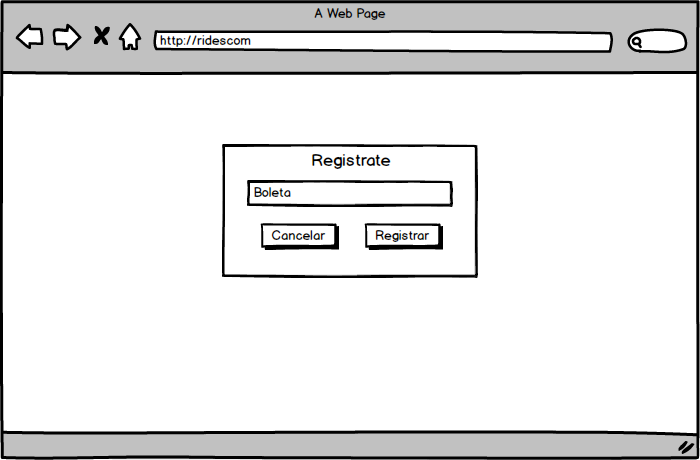
\includegraphics[width=10cm, height=6cm]{Imagenes/Disenos/VistasBorradas/p1_Registro.png}
		\caption{Registro para los alumnos.}
	\end{figure}
	
	\begin{figure}[hbt!]
		\centering
		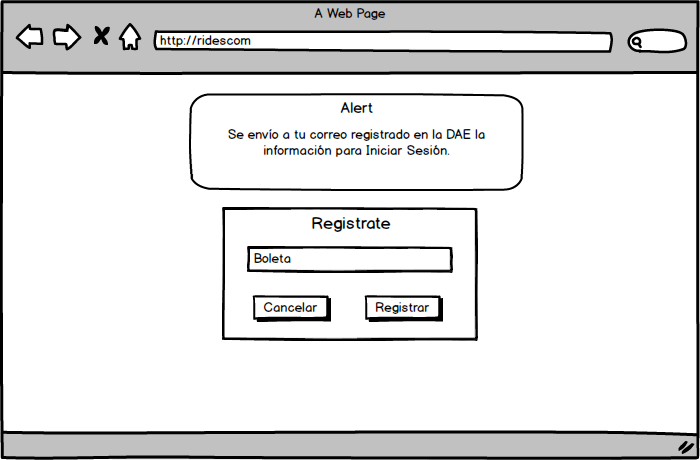
\includegraphics[width=10cm, height=6cm]{Imagenes/Disenos/VistasBorradas/ConfirmacionRegistro.png}
		\caption{Confirmación registro para los alumnos.}
	\end{figure}
	
	\begin{figure}[hbt!]
		\centering
		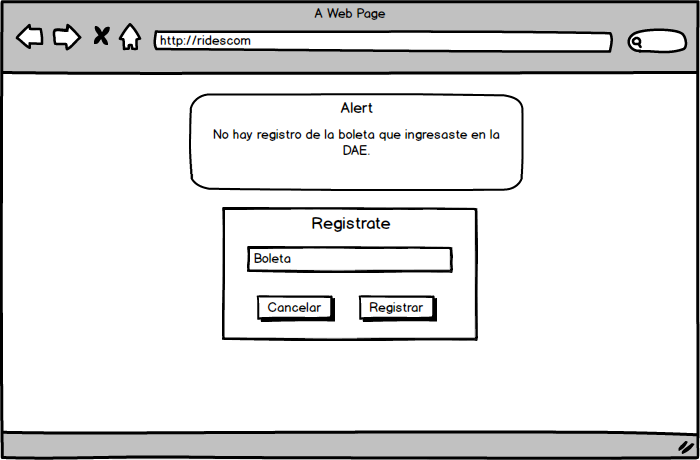
\includegraphics[width=10cm, height=6cm]{Imagenes/Disenos/VistasBorradas/p3RechazoRegistro.png}
		\caption{Rechazo registro para los alumnos.}
	\end{figure}

	\begin{figure}[hbt!]
		\centering
		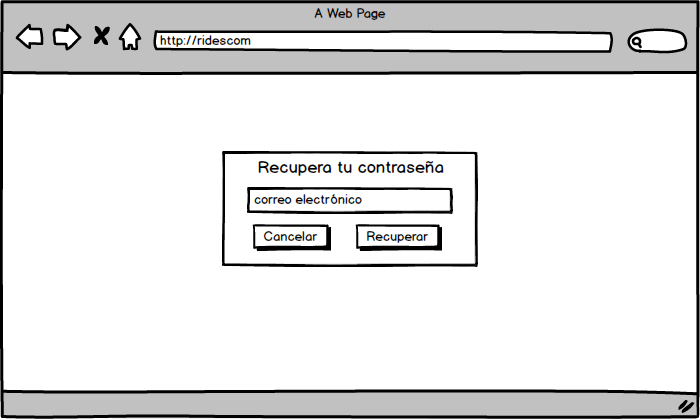
\includegraphics[width=10cm, height=6cm]{Imagenes/Disenos/VistasBorradas/p5Recuperarcontrasena.png}
		\caption{Recuperar contraseña para los alumnos.}
	\end{figure}

	\begin{figure}[hbt!]
		\centering
		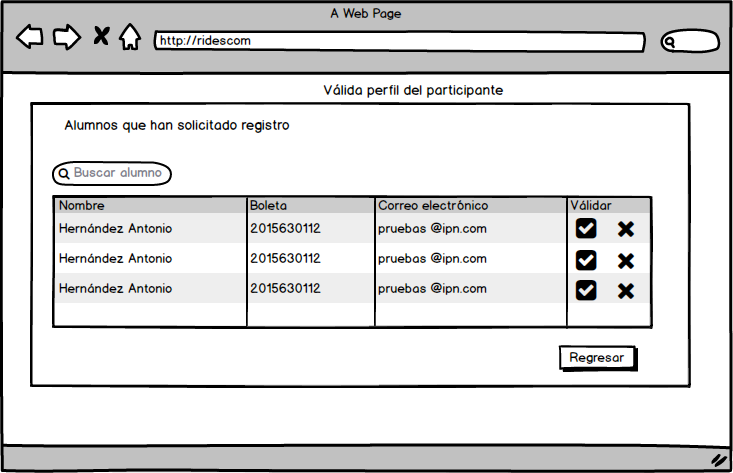
\includegraphics[width=10cm, height=6cm]{Imagenes/Disenos/VistasBorradas/p18ValidaPerfil.png}
		\caption{Validar perfil de los alumnos.}
	\end{figure}
	\pagebreak

	